% TODO: Dodělat
\documentclass{szzclass}
\usepackage[czech]{babel}
\usepackage{hyperref}
\usepackage{dependencies/szz-code}

% \subject{TJV}
% \code{BI-WSI-SI-28}
% \topic{JDBC v podnikových aplikacích: popis JDBC obecně, popis dat datového zdroje (DataSource), nastavení datových zdrojů v aplikačním serveru (JDBC Connection Pool, JDBC Resources).}

\begin{document}

\section{JDBC Java Database Connectivity}
\begin{itemize}
\item Java rozhraní pro připojení k relační databázi
\item Součástí přímo Java SE už od verze 1.1
\item Umožňuje vytvořit takzvané spojení (connection) s databází
\item Přes toto spojení lze pak spouštět dotazy SELECT, CREATE, INSERT, UPDATE a DELETE.
\item JDBC je pouze obecné rozhraní. Pro připojení ke konkrétnímu typu databáze (MySQL, PostgreSQL....) je potřeba takzvaný driver.
\item JDBC Driver realizuje spojení s konkrétní databází → implementuje JDBC interface
\end{itemize}
\begin{figure}[h!]

\includegraphics[width=0.95\textwidth]{topics/bi-wsi-si-28/images/image1.png}
\end{figure}

\section{Připojení se k DB}
Nejdříve se k databázi připojíme (pozn.: try-with-resources funguje od Javy 7) pomocí třídy \mintinline{java}{DriverManager}. Před Javou 6 bylo třeba explicitně definovat třídu driveru a načíst ji.

\begin{minted}[breaklines]{java}
try (Connection conn = DriverManager.getConnection(
     "jdbc:mysql://localhost/mydb",
     "myLogin",
     "myPassword")) {

  // zde používáme vytvořené spojení

}  // Java VM se postará o uzavření spojení
\end{minted}


Využití DriverManageru je vcelku nepraktické (musíme být v try bloku), a proto vznikl DataSource. Jedná se o interface, která vrací stejnou Connection jako DriverManager. Vývojáři DB musí poskytovat konkrétní implementaci DataSource. Connection lze získat bez parametrů nebo s pomocí dvojice \uv{jméno a heslo}.

\begin{minted}[breaklines]{java}
com.dbaccess.BasicDataSource ds = new com.dbaccess.BasicDataSource();
ds.setServerName("mujserver");
ds.setDatabaseName("mojedatabaze");

// Metoda odstinena od konkretniho driveru → polymorfismus
public void doThings(DataSource ds) {
  Connection con = ds.getConnection("user", "psswd");
}
\end{minted}

Detaily připojení tak nemusí být napevno v aplikaci. DriverManager dále nabízí connection pooling (viz níže).

\section{Práce s DB}
Příkazy se vykonávají pomocí třídy Statement.

\begin{minted}[breaklines]{java}
try (Statement stmt = conn.createStatement()) {
  stmt.executeUpdate("INSERT INTO table VALUES ('neco')");
}
\end{minted}

Existuje pak i PreparedStatement, do kterého lze dodávat argumenty dynamicky.

\begin{minted}[breaklines]{java}
try (PreparedStatement ps = conn.prepareStatement(
     "SELECT * FROM person WHERE name = ? AND age = ?")
) {
    ps.setString(1, "Poor Yorick");
    ps.setInt(2, 90);
}
\end{minted}

Návratová hodnota je \mintinline{java}{ResultSet}. Je to takový převlečený návrhový vzor \mintinline{java}{Cursor ~ Iterator}.
Můžeme s pomocí něj iterovat přes řádky výsledků a podle indexů sloupce si sahat na jednotlivé hodnoty.

\begin{minted}[breaklines]{java}
try (Statement stmt = conn.createStatement();
     ResultSet rs = stmt.executeQuery("SELECT * FROM person")
) {
  while(rs.next()) {
    String personName = rs.getString(1); // index sloupce
    int personAge     = rs.getInt(2);
  System.out.printf("Osoba: %s (%d)\n", personName, personAge);
  }
}
\end{minted}

Dále lze pomocí příznaků specifikovat, jestli iterace může být pouze jednosměrná nebo oboustranná.

Jeden příkaz znamená jeden atomický dotaz do databáze. V rámci jedné transakce lze ale vykonat více příkazů. Ovlivňuje to metoda \mintinline{java}{Connection#setAutoCommit(boolean)}. Pokud nastavíme autocommit na false, tak je potřeba transakci ručně odeslat - \mintinline{java}{Connection#commit()}.

\begin{figure}[h!]
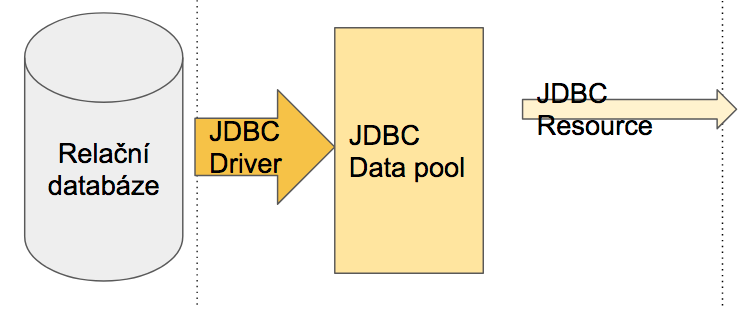
\includegraphics[width=0.95\textwidth]{topics/bi-wsi-si-28/images/image2.png}
\end{figure}

\section{JDBC Connection pooling}
Problém - pro každé vykonání dotazu je třeba se k databázi připojit. Připojení stojí nějaký čas a není dobré se neustále připojovat a odpojovat. Connection pooling zajišťuje, že připojení proběhne na začátku a zachová se i po vykonání dotazu. Pro další dotaz je existující připojení znovupoužito.

Connection pooling probíhá v Javě automaticky, pokud je využit \mintinline{java}{DataSource}. Podpora musí být na straně implementace této \mintinline{java}{interface}. JDBC 3.0 API Framework specifikuje sadu rozhraní, které musí být implementovány.
\begin{itemize}
\item \mintinline{java}{ConnectionPoolDataSource} - implementace od autorů databází slouží jako factory, která vytváří PooledConnection
\item \mintinline{java}{PooledConnection} - řídí připojení k databázi
\item \mintinline{java}{ConnectionEventListener} - listener změn v připojeních k DB
\end{itemize}

Nastavení Connection poolu se v TJV dělalo přes Glassfish. Na localhost webu se zadaly přihlašovací údaje do databáze, adresa databáze atp.

Jak na to - viz video \url{https://youtu.be/f1z-3zlkXj8?t=2m27s }

\section{JDBC Resource}
Poskytuje prostředky pro připojení k databázi. Pro vytvoření je potřeba speficikovat Connection pool, se kterým bude spjat. Má vlastní jméno (JNDI name), které dle konvence začíná “jdbc/”.

Přístup ke zdroji lze získat přes \mintinline{java}{InitialContext}:

\begin{minted}[breaklines]{java}
InitialContext ic = new InitialContext();
DataSource source = (DataSource) ic.lookup("jdbc/my_resouce_name");
\end{minted}

\section{Zdroje}
Celý převzato z \url{https://docs.google.com/document/d/1Wfd-xg3CgY6YCLi15wh3ngDN0sPNNcg3bplWePlXTwM/edit#}
\begin{itemize}
\item JDBC Polling podrobně \url{https://www.progress.com/tutorials/jdbc/jdbc-jdbc-connection-pooling }
\item JDBC Resources \url{https://docs.oracle.com/cd/E19316-01/820-4335/ablih/index.html }
\item Připojení k JDBC Resource \url{https://docs.oracle.com/javase/tutorial/jdbc/basics/sqldatasources.html }
\item BI-TJV 4. Přednáška \url{https://docs.google.com/presentation/d/12jr7jnWbx_S4sIwLd0v9HmUyX1uuAP3-z6HOdIDp7WA/edit }
\end{itemize}
\end{document}
